\documentclass[11pt]{article}

\pdfminorversion=4

% use packages
\usepackage[utf8]{inputenc}
\usepackage{amsmath}
\usepackage{amsthm}
\usepackage{amsfonts}
\usepackage{amscd}
\usepackage{amssymb}
\usepackage{natbib}
\usepackage{url}
\usepackage[table,xcdraw,usenames]{xcolor}
%\usepackage[usenames]{color}

\usepackage{graphicx}
\usepackage{subcaption}
\usepackage{mathtools}
\usepackage{enumitem}
\usepackage{authblk}
\usepackage{bm}
\usepackage{comment}
\usepackage{pdfpages}

\usepackage{hyperref}
\usepackage{caption}
\usepackage{float}
%\usepackage[caption = false]{subfig}
\usepackage{tikz}
\usepackage{multirow}
\usepackage[linesnumbered, ruled,vlined]{algorithm2e}
\usepackage{pdflscape}
\usepackage{etoolbox}

%\AtBeginEnvironment{align}{\setcounter{equation}{0}} % https://tex.stackexchange.com/questions/349247/how-do-i-reset-the-counter-in-align

% margin setup
\usepackage{geometry}
\geometry{margin=0.8in}

% function definition
\newcommand{\V}{\textbf{V}}
\newcommand{\weight}{\pi}
\newcommand{\ret}{\textbf{r}}
\newcommand{\y}{\textbf{y}}
\newcommand{\w}{\textbf{w}}
\newcommand{\x}{\textbf{x}}
\newcommand{\dbf}{\textbf{d}}
\newcommand{\X}{\textbf{X}}
\newcommand{\Y}{\textbf{Y}}
%\newcommand{\L}{\textbf{L}}
\newcommand{\Hist}{\mathcal{H}}
\newcommand{\Prob}{\mathbb{P}}
\def\mbf#1{\mathbf{#1}} % bold but not italic
\def\ind#1{\mathrm{1}(#1)} % indicator function
\newcommand{\simiid}{\stackrel{iid}{\sim}} %[] IID 
\def\where{\text{ where }} % where
\newcommand{\indep}{\perp \!\!\! \perp } % independent symbols
\def\cov#1#2{\mathrm{Cov}(#1, #2)} % covariance 
\def\mrm#1{\mathrm{#1}} % remove math
\newcommand{\reals}{\mathbb{R}} % Real number symbol
\def\t#1{\tilde{#1}} % tilde
\def\normal#1#2{\mathcal{N}(#1,#2)} % normal
\def\mbi#1{\boldsymbol{#1}} % Bold and italic (math bold italic)
\def\v#1{\mbi{#1}} % Vector notation
\def\mc#1{\mathcal{#1}} % mathical
\DeclareMathOperator*{\argmax}{arg\,max} % arg max
\DeclareMathOperator*{\argmin}{arg\,min} % arg min
\def\E{\mathbb{E}} % Expectation symbol
\def\mc#1{\mathcal{#1}}
\def\var#1{\mathrm{Var}(#1)} % Variance symbol
\def\checkmark{\tikz\fill[scale=0.4](0,.35) -- (.25,0) -- (1,.7) -- (.25,.15) -- cycle;} % checkmark
\newcommand\red[1]{{\color{red}#1}}
\def\bs#1{\boldsymbol{#1}}
\def\P{\mathbb{P}}
\def\var{\mathbf{Var}}
\def\naturals{\mathbb{N}}
\def\cp{\overset{p}{\to}}
\def\clt{\overset{\mathcal{L}^2}{\to}}

\setcounter{tocdepth}{4}
\setcounter{secnumdepth}{4}

\newtheorem{corollary}{Corollary}
\newcommand{\ceil}[1]{\lceil #1 \rceil}
\newcommand{\norm}[1]{\left\lVert#1\right\rVert} % A norm with 1 argument
\DeclareMathOperator{\Var}{Var} % Variance symbol

\newtheorem{cor}{Corollary}
\newtheorem{lem}{Lemma}
\newtheorem{thm}{Theorem}
\newtheorem{defn}{Definition}
\newtheorem{prop}{Proposition}
\theoremstyle{definition}
\newtheorem{remark}{Remark}
\hypersetup{
  linkcolor  = blue,
  citecolor  = blue,
  urlcolor   = blue,
  colorlinks = true,
} % color setup

% proof to proposition 
\newenvironment{proof-of-proposition}[1][{}]{\noindent{\bf
    Proof of Proposition {#1}}
  \hspace*{.5em}}{\qed\bigskip\\}
% general proof of corollary
  \newenvironment{proof-of-corollary}[1][{}]{\noindent{\bf
    Proof of Corollary {#1}}
  \hspace*{.5em}}{\qed\bigskip\\}
% general proof of lemma
  \newenvironment{proof-of-lemma}[1][{}]{\noindent{\bf
    Proof of Lemma {#1}}
  \hspace*{.5em}}{\qed\bigskip\\}

\allowdisplaybreaks

\title{Forecast Adjustment Under Shocks: A Unification}
\author{David P. Lundquist\thanks{davidl11@ilinois.edu}, Daniel J. Eck\thanks{dje13@illinois.edu} }
\affil{Department of Statistics, University of Illinois at Urbana-Champaign}
\date{\today}

\begin{document}

\maketitle

\begin{abstract} 
Structural shocks to time series may give an observer reason to doubt the credibility of the default forecasting function.  This work systematizes and unifies the rich landscape of model adjustment and model correction methods, with a special focus on forecast adjustment under the presence of shocks.  We demonstrate the usefulness of similarity-based methods in forecasting and present several specific models that can benefit, along with formal results for some of those special cases.

\end{abstract}





\section{Introduction}\label{Introduction}

\textbf{Plan}

What the paper should do
\begin{itemize}
  \item Introduce an existing diffuse set of approaches to adjusting forecasts (\ref{Introduction})
  \item Explain when/how similarity can help us forecast. \ref{meaning_use}
  \item distinguish the method from various tools that inspired it (\ref{Introduction})
  \item show a few special cases, both examples and formal results (\ref{special_cases})
  \item discuss limitations of the method (\ref{Limitations})
  \item propose extensions (\ref{Extensions})
\end{itemize}

What the paper should NOT do

\begin{itemize}
  \item Wade too deeply into distance-based weighting details.  State that it's simply one way to do it.  Allude to \cite{lin2021minimizing,lundquist2024volatility}.
  \item wade too deeply into any of the special cases
  \item Tackle non-scalar random quantities (density forecasts, etc)
  \item Forecast combination

\end{itemize}

For various modeling and prediction tasks in time series and panel data, the salient challenge is not predicting when an event will occur but what its key properties will be.  In the familiar case of scalar time series, those properties can include its post-event direction, moments, sign, magnitude, duration, and correlation structure, all over an arbitrary horizon or perhaps multiple horizons. This is not to say that predicting the arrival of an event is easy. In some cases, it may be difficult or impossible, and therefore preparing for an antipicated shock is the best one can hope for.

This work focuses on model adjustment amid structual shocks that undermine the reliability of the  model at hand.  Forecasting under anticipated shocks raises unavoidable questions: should the forecast model be abandoned in favor of a discretionary or ad-hoc or one-off adjustment?  Does the does the discretion of a forecaster rule out a quantitative method for making the adjustment?  What is the ultimate purpose of the adjustment, and how it is to be used?  For how long is the adjustment necessary or reliable?

Herein we systematize and unify a range of conceptual approaches and tools that have developed across the broad ecosystem of the econometric and forecasting literatures.  Additionally, we delineate a specific type of forecasting task called post-shock forecasting, which we broadly define as forecasting under a known shock.

Forecast model adjustment, known most widely perhaps by the term intercept-correction, has received the most attention in several articles and book chapters \citep{hendry1994theory,clements1996intercept,clements1998forecasting}.  Of special importance is the distinction between discretionary and automated intercepts corrections. \cite{hendry1994theory} define scalar intercept corrections to be automated when they follow the simple rule of adding an estimation residual $e_{t}$ to subsequent (possibly but not necessarily all) forecasts $\hat f_{t+1},\hat f_{t+2},...$.  This procedure can colloquially referred to as setting the model back on track \citep{hendry1994theory}.  In \cite{hendry1994theory}, after recounting the bipartite division of interception corrections in discretionary and automated varieties, the authors present a six-way taxonomy of information that a modeler possesses at the time a forecast is made.  The authors also consider structural change in the data-generating process during the forecast period, including as early as the first point in the forecast period (specifically in the autoregressive structure), as well as what is for them the more interesting case: structural change between $T^{*}-1$ and $T^{*}$.  This current work finds both cases interesting.  What if we could predict well the intercept shift that occurs between $T^{*}$ and $T^{*}+1$?

Post-shock forecasting procedures have been explored in \cite{lin2021minimizing,lundquist2024volatility}, where the AR(1) and GARCH($m,s$) cases, respectively, are treated.  Both works target additive parameters in scalar time series, predicting those random effects by aggegating information from other time series.  The authors leave several stones unturned, including a more general, dare say comprehensive treatment of how to forecast under any sort of shock.

A practitioner interested in forecast adjustment can choose between procedures that discretionary or automated, a variety of choices for the collection of data assembled to perform the correction, whether the data is internal (i.e. from the time series itself) or external, the parametric term to be corrected (e.g. intercept, coefficients), if any, as well as the correction function (i.e. the mapping from the data to the corrective term), including the weighting applied to the assembled data (e.g. Nearest-Neighbor, arithmetic mean, kernel methods).

The procedure presented herein is a discretionary procedure for intercept correction that integrates data internal or external to the time series under study in a systematic manner.  The correction function uses an optimization step inspired by the causal inference literature.  Outside of \citet{lin2021minimizing,lundquist2024volatility}, we are not aware of prior work that both introduces a parametric specification for nonzero errors and introduces a procedure for weighting appropriately the nonzero errors of similar shocks occurring outside the time series under study.  We are also not familiar with any prior work that attempts to account for anticipated nonzero errors using an a parametric adjustment, i.e., a ``correction function''.  

The structure of this manuscript is as follows.  We first provide a  review of several disparate time series literatures, including intercept correction, model-evaluation, and similarity-based forecasting.  We then provide a canonical setting in which we attempt to focus our work.  This setting will be presented at a level of generality that showcases the broad applicability of our method.  We then introduce the method from a global perspective, abstracting away from familiar applications.  We then show several specific applications, including novel applications that cannot be found elsewhere in the literature.  We close with a discussion, including possible extensions.

\subsection{Here is what we are not doing}

\subsubsection{Intercept Correction}\label{intercept_correction}
\subsubsection{Forecast Combination}
what we are talking about here is not forecast combination, but there may be, nevertheless, a role for forecast combination: combining the forecasts generated by small differences in covariate and/or donor choice, as is done in \cite{lundquist2024volatility}. \\

\subsubsection{Tackle non-scalar random quantities (density forecasts, etc)} 

\begin{itemize}
  \item Function forecasts
  \item Binary Outcome Forecasts
  \item Density Forecasts
  \item Quantile Forecasts
\end{itemize}
\subsection{History of and Motivation for Intercept Correction}
See Clements and Hendry
\subsubsection{Setting levels back on track}

We discussed this above in Section \ref{intercept_correction}.

\subsubsection{Mismeasured data}

Mismeasured data is discussed in \cite[p. 166]{hendry1994theory} as a motivator for intercept correction.  Could similarity-based correction help?  Here is an idea: if we believe that our most recent measurement of the series is noisy, we can disregard the point itself and instead take a convex combination of that point and the \cite{lin2021minimizing}-style prediction based on aggregation.

Quinton-Guerrera and Zhong \cite{guerron2017macroeconomic} - concerned with correcting $\beta$ using similarity\\

\subsubsection{Motivation from model evaluation}

Part of the reason for correcting a model springs from the way we evaluate model performance.
Evaluating a Model by Forecast Performance \cite{clements2005evaluating}
\begin{enumerate}

  \item   unconditional versus conditional, models;
  \item internal versus external standards;
  \item checking constancy versus adventitious significance;
  \item ex ante versus ex post evaluation (skip this one?);
  \item 1-step versus multi-horizon forecasts -- this is a relevant question to ask in the context of post-shocking forecasting: should we correct the earliest forecast and then allow the shock to propagate, or should we just correct each term in the horizon, h=1, 2,..., H?
  \item in-sample fixed coefficients versus continuous updating
\end{enumerate}

Here is the argument: if we are going to judge a model by forecast performance, we need to entertain the possibility that the model may breakdown and that our pre-breakdown-based criteria for model performance will be invalidated.

\subsection{The Meaning and Use of Similarity}\label{meaning_use}
Hume? Cite Israeli authors, if so.\\

The notion of similarity appears in various statistical contexts, including matching, synthetic control, nearest-neighbor methods, not to mention the massive area of approximation theory.  The uses of similarity are too sprawling to recount in detail.  Below we talk about how it could matter in this work.

Similar, in the strong sense, could mean that a shared DGP exists. It could mean similar in the covariates that parameterize the shocks.  It matters where we look for similarity and how we estimate similarity.

Quantitative ways of determining similarity include matching a target object to other objects along one or more variables, where exact matches may be likely or may be statistically impossible.  In metric spaces, the notion of a metric that quantifies nearness is crucial to fundamental concepts of proximity.  This suggests an optimization problem such that, for any target object $Q$, the search for similarity means a search for an approximator $A$ s.t. $\delta(Q,A)$ is smallest, where $\delta$ is an appropriate metric.

Asymmetric distance functions (which are of course not metrics) are useful when we want to explore differences between donors and weight different contributors to that function differently.

What about qualitative ways of determining similarity?  In \cite{lundquist2024volatility}, donors are identified by matching the qualitative aspects of the shock in the time series under study to shocks previously witnessed in other series.  Only after the donor pool has been identified based on qualitative facts about the shocks is there a role for quantative tools.

\section{Setting}\label{Section}

\textcolor{red}{It's unclear how much I can show the reader, given that I want this to be general.}

In order to introduce the general framework for adjusting forecasts under shocks, we provide an illustration.  In Figure [decide on which figure to include] %\ref{fig:motivating_piece_convex_combination}, 
we show how the aggregation of estimated excess volatilities from donors in the donor pool works when the correction function is a specially-chosen convex combination of fixed effects from the donor pool.  Our method assumes a credible, parsimonious parameterization in which the shock is an affine transformation of several key covariates.  The key intuition behind this shock parameterization is that as the strength of the linear signal increases relative to the idiosyncratic error, the estimation of these effects increases in accuracy.  From this, it follows that the aggregated shock estimate increases in accuracy.

\textcolor{red}{The preceding information is correct.  However, it comes from the previous paper, so it needs to be changed to suit the style of the current paper.}

\subsection{A shock between discrete time points}
In this work, we will be focused on shocks that occur strictly between two discrete time points.  This raises an important terminological point.  ``Shocks", in econometric literature, can be structural or idiosyncratic, permanent or transitory, supply-related or demand-related, and so forth.  The taxonomy is vast.

\subsection{Formal Modeling Setup}

  \begin{figure}[h!]
    \begin{center}
      \begin{tikzpicture}
        \node[anchor=south west,inner sep=0] at (0,0) {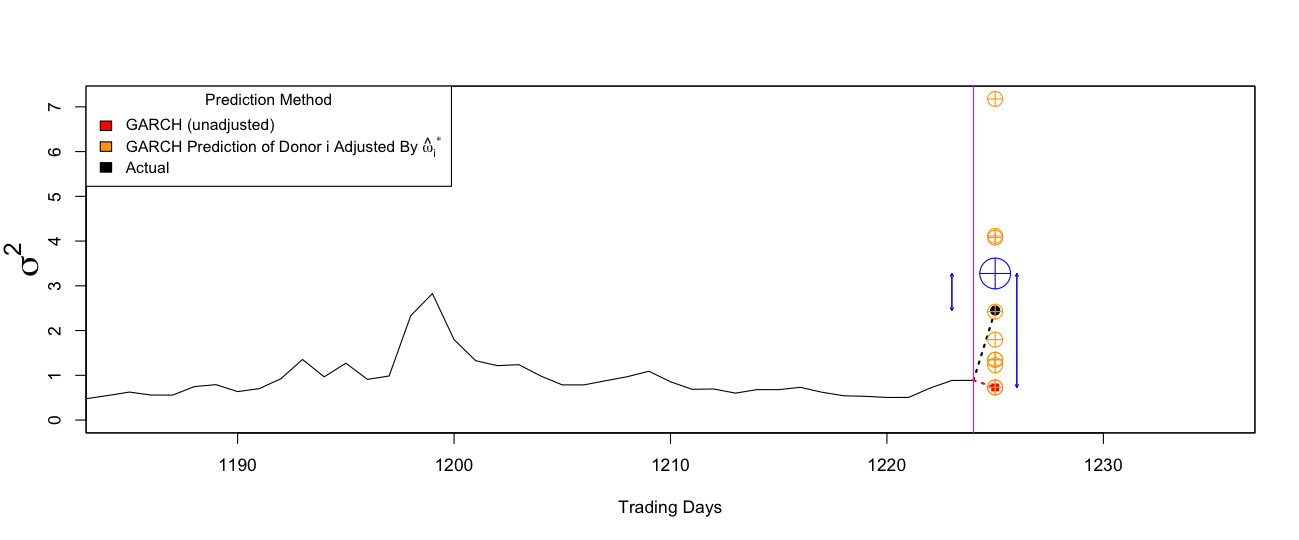
\includegraphics[width=\textwidth]{simulation_plots/motivating_piece_convex_combination.png}};
        % \draw[red,ultra thick,rounded corners] (7.5,5.3) rectangle (9.4,6.2);
        % \node[draw,text width=4.45cm] at (9.8,3.2) {$\textcolor{blue}{\hat\sigma^{2}_{adjusted} = \hat\sigma^{2}_{unadjusted} + \hat\omega^{*}}$ };
        % \node[draw,text width=2.62cm] at (14.8,2.8) {$\textcolor{blue}{\hat\omega^{*} = \sum^{n+1}_{i=2}\pi_{i}\hat\omega^{*}_{i}}$ };    
        
    \end{tikzpicture}
      \caption{The simulated time series experiences a volatility shock between trading days 1,656 and 1,657.  The GARCH prediction, in red, fails even to approach the volatility spike at $T^{*}+1$, as do several adjusted predictions, which are orange.  In contrast, the GARCH forecast adjusted by $\hat\omega^{*} = \sum^{n+1}_{i=2}\pi_{i}\hat\omega^{*}_{i} $, a convex combination of the estimated shocks in the donor pool, achieves directional correctness as well as a smaller absolute loss in its prediction.  The pink vertical line serves to indicate the adjustment of size $\hat\omega^{*}$ that allows the blue bullseye to approach more closely the ground truth.}    \label{fig:motivating_piece_convex_combination}
   
      \end{center}
    \end{figure}

We will suppose that a researcher has multivariate time series data $\y_{i,t} = (r_{i,t}$, $\x_{i,t}$), $t = 1,$ $\ldots,  T_i$, $i = 1, \ldots, n+1$, where $r_{i,t}$ is scalar and $\x_{i,t}$ is a vector of covariates such that $\x_{i,t}|\mathcal{F}_{i,t-1}$ is deterministic.  Suppose that the analyst is interested in forecasting $r_{1,t}$, the first time series in the collection, which we will denote \textit{the time series under study}.   We assume the following general data-generating process

\begin{align*}
  &y_{t} = F(\mathcal{F}_{t-1}) + \epsilon_{i,t}\\
\end{align*}
where $\epsilon_{i,t}$ is mean-zero and uncorrelated across time and donors.



Note that this specification above is capacious enough to include data-generating processes of the form 

\begin{align*} 
  y_{t} = \log{Y_{i,t}} = \log{a_{i}Y_{i,t-k}\epsilon_{i,t}} = \log{a_{i}} + \log{Y_{i, t-k}} + \log{\epsilon_{i,t}}
\end{align*}
with $k\geq1$ and all variables on the right-hand side supported on $\mathbb{R}^{+}$.

We require that each time series $\y_{i,t}$ is subject to an observed news event following $T^*_i \leq T_{i} + 1$ and before witnessing $T^*_i+1$.  Our reasons for this will now become clear.

We will suppose further that $F(\mathcal{F}_{t})$ includes a random effect $\lambda_{t}$, allowing us to write

\begin{align*}
  &y_{t} = F(\mathcal{F}_{t-1}) + \epsilon_{i,t} = F^{D}(\mathcal{F}_{t-1}) + \x_{t}^{T}\lambda_{t} + \epsilon_{i,t}\\
\end{align*}



\section{Model Adjustment Using Similarity-Based Parameter Correction: A Global Overview}

In this section, we introduce and discuss a particular approach to model adjustment that is motivated by the circumstances laid out in Section \ref{Section}.  It may not yet be clear what is essential and what is not.  Here we make that clear.

\subsection{The six essential elements of similarity-based parameter correction
}

\textcolor{red}{Should I just use OLS as an example throughout all six?}

Most fundamentally, the method requires a random object (indexed over time, of course) that obeys a specification with additive errors, or, at the very least, a specification that can be transformed to have additive errors.\footnote{Emphasize that there is a non-parametric version of the above: for example, one can use LSTM to predict each of the donor shocks, and then the residuals (or transformations of those residuals, e.g. to percentages) of those n models can be weighted to arrive at a correction term.}  This requirement is suitably weak, so as to include models that are not linear or not linear in each of their parameters.  It also includes objects that multidimensional, hail from non-Euclidean probability spaces, like some function spaces.

Second, the method requires a model family that is shared across all units.  This ensures that in the estimation of structural shocks in the donor pool, the estimators will enjoy similar properties that will produce a good aggregrated shock estimator.

Third, the data-generating processes of the units must include a correction term that serves as the basis of the aggregation.  The correction term must have a parametric specification.  The correction term must be estimable in each time series(?).   It may depend on external covariates, as we see in \cite{lin2021minimizing} and \cite{lundquist2024volatility}.

Fourth, there must exist a reliable estimation procedure for the units that obey the common family of data-generating processes.  In this case, reliable means several things.  It means that the estimation procedure must produce a credible description of each data-generating process, so as to aid in estimating the correction term in each unit.  That may mean the estimators have low variance, and it may also mean that the estimation procedure is robust, to some degree, to misspecification bias.  However, in theory, the lack of these properties is not harmful to the method unless the lack of these properties harms the correction term's estimation.

When we use fixed effect estimation (under ordinary assumptions), we can construct confidence intervals for the fixed effect estimates, and then assuming independence, we can get confidence intervals for convex combinations of fixed effect estimates.

Fifth, there must exist a reliable procedure for the correction term in each unit.  Again, here we care about low variance as well as robustness to misspecification.  The correction term could be as simple as fixed effect estimation.  It could depend upon external covariates.

This might not be straightforward.  Some models like GARCH, for example, might deliver very noisy estimates for indicator variables that occur just once.  When will it be as simple as a fixed effect?  When will it be something besides a fixed effect?

Sixth and finally, there must exist a correction function (presumably based on the correction term) that maps data from the donor pool to the \textit{predicted} correction term in the time series under study based on some notion of similarity.  It could depend upon external covariates.

\section{Methodology for Similarity-based Parameter Correction}
\subsection{Forecasting}

We now turn to the next section, where $\textbf{V}_{t}$ is employed in a procedure to arrive at a forecast adjustment. For illustration, we present two one-step-ahead forecasts for the time series under study. The first is the unadjusted GARCH forecast. The second is the adjusted forecast, which differs by the additive term $\hat\omega^{*}$ that is computed via our distance-based weighting procedures.  These forecasts are: 

\textcolor{red}{These should be kept, with appropriate things changed.}

\begin{align*}
  %\text{Forecast 1: } 
  & \hat\sigma^{2}_{unadjusted, T_{1}^{*}+1} = \hat\E[|\mathcal{F}_{T_{1}^{*}}] && = && ,\\
  %\text{Forecast 2: } 
  & \hat\sigma^{2}_{adjusted,T_{1}^{*}+1} = \hat\E[|\mathcal{F}_{T_{1}^{*}}] + \hat\omega^{*} && = && \text{ .}
\end{align*}

\subsection{Shock Estimators}
    \label{Shock_Estimators}
   
    The problem of aggregating estimated donor shocks begins with the data constraints.  Let us first introduce useful notation.  Let $\hat\omega^{*}_{i,*}$ denote the shock estimate for donor $i$ that is obtain via an indicator variable over time points $T_{i}^{*}+1,...,T_{i}^{*}+L_{i,vol}$.  That estimation procedure is justified by the assumption that at each nonzero shock point, the shocks will differ but will be equal in distribution.  
    
    Taking the estimated shocks as a given, we observe the pair $(\{\hat\omega^{*}_{i,*}\}^{n+1}_{i=2},\{\textbf{v}_{i}\}^{n+1}_{i=2})$.  Let $\Delta^{n} = \{\pi \in \mathbb{R}^n: \sum_{i=1}^n \pi_i = 1, \pi_i \geq 0 \, i = 1,...,n\}$.  We wish to recover weights $\{\weight_{i}\}^{n+1}_{i=2} \in \Delta^{n}$ leading to favorable forecasting properties.  These weights are used to define and compute an aggregate shock estimate 
\begin{equation} \label{adjustment}
	  \hat\omega^{*} = \sum^{n+1}_{i=2}\weight_{i}\hat\omega^{*}_{i,*},
\end{equation}
    which will be taken to be our forecast adjustment term.  Since the weights $\{\weight_{i}\}_{i=2}^{n+1}$ are computed using $\mathcal{F}_{T^{*}_{i}}$, the set $\{\weight_{i}\}_{i=2}^{n+1}$ is deterministic and observed, $\textit{modulo}$ any stochastic ingredient in the numerical methods employed to approximate $\x_{1,T^{*}+1}$ using a convex combination of donor covariates.  We say more about the properties of the shocks $\omega^{*}_{i,T_{i}^{*}+1},...,\omega^{*}_{i,T_{i}^{*}+L^{vol}_{i}}$ in section $\ref{SVF_properties}$. 

    Following \citet{abadie2003economic,abadie2010synthetic,lin2021minimizing}, let $\|\cdot\|_{\textbf{S}}$ denote any semi-norm on $\mathbb{R}^{p}$, and define
    \begin{align*}
    \{\pi\}_{i=2}^{n+1} = \argmin_{\pi}\|\x_{1,T^* + 1} - \V_{T^* + 1}\pi\|_{\textbf{S}}. 
    \end{align*}
In the forecast combination literature, it is of interest whether the weights employed to aggregate forecasts strive toward and meet various optimality criteria \citep{timmermann2006forecast,wang2023forecast}.  In our endeavor, there are at least two senses of optimal weights that one might be interested in.  First, we can think of optimal weights as a set $\{\weight_{i}\}_{i=2}^{n+1}$ such that $\omega_{1} = \sum^{n+1}_{i=2}\weight_{i}\hat\omega_{i,*}$, i.e., $\omega_{1}$ is recovered perfectly, as it belongs to convex hull of the estimated shocks. However, $\omega_{1}$ is never revealed to the practitioner, and hence there is no way of verifying the extent to which this condition is satisfied.

\subsection{Shock propagation and estimation accuracy}
Consider \cite{lundquist2024volatility}, in which a real world example shows how volatility can be forecasted following surprising election outcomes.  There, the estimation of fixed effects is done around elections in a donor pool.  That means that for each past election or poll, etcetera, the method must accurately estimate the surprise-induced volatility boost.  That means picking a window around such an effect.
    
\subsection{How is the proposed method distinct from existing tools?}

\subsection{Relaxation of Assumptions}
\subsubsection{How important is a shared DGP?}

The assumption of a shared family can be relaxed in certain circumstances.  For example, if a certain donor is not like the time series under study with respect to the covariates, then the lack of a shared family will not matter much.
\subsection{We can use the method on latent time series}
See \cite{lundquist2024volatility}

\section{Formal Properties and Model-Specific Considerations}\label{special_cases}

 


\subsection{ARIMA}
\cite{lin2021minimizing}
\subsection{GARCH}
We briefly highlight the findings of \citep{lundquist2024volatility}.
\subsection{HAR}
\begin{figure}[h!]
  \begin{center}
    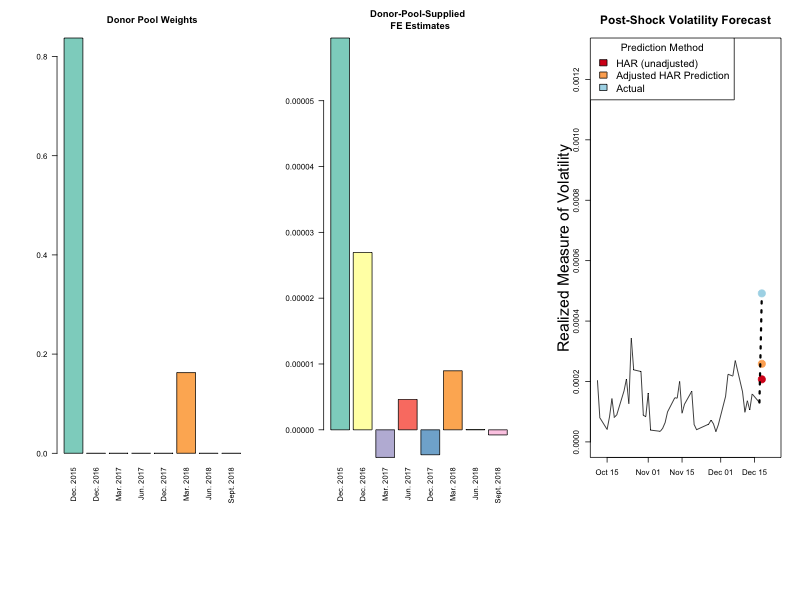
\includegraphics[scale=.4]{real_data_output_plots/savetime_SatJun151644072024__^VIX-^IRX-^XAU_^VIX_2018-12-18-2015-12-15-2016-12-13-2017-03-14-2017-06-13-2017-12-12-2018-03-20-2018-06-12-2018-09-25.png}
    \caption{Volatility series of six i.i.d. GARCH processes, each of which experiences a volatility shock, indicated with a red vertical line, at a uniformly distributed point in the set $\{756,...,2520\}$ of trading days, corresponding to between 3 and 10 years of daily trading data.}
    \label{fig:six_plots}
    \end{center}
  \end{figure}

\subsection{VAR}
Many time series, especially macroeconomic time series, naturally arise as constituents of groups of dependent variables that interact across time.
\subsection{LSTM/GRU}

Here we demonstrate the tremendous capaciousness of our method by applying it to predictions generated by a pair of non-parametric forecasting functions, Long Short Term Memory and GRU.  We will re-examine an application found in \cite{lin2021minimizing}.

We borrow code from \cite{Brownlee_2022}

\begin{itemize}
  % \item \href{https://www.r-bloggers.com/2021/04/lstm-network-in-r/#google_vignette}{a}
  % \item \href{https://sharmasaravanan.medium.com/an-implementation-guide-for-lstm-in-r-2347e4118a2c}{b}
  % \item \href{https://search.r-project.org/CRAN/refmans/TSdeeplearning/html/GRU_ts.html}{c}
  % \item \href{https://medium.com/codex/time-series-prediction-using-lstm-in-python-19b1187f580f#:~:text=In%20conclusion%2C%20LSTM%20models%20are,in%20your%20data%20science%20toolkit.}{d}
  \item \href{https://machinelearningmastery.com/time-series-prediction-lstm-recurrent-neural-networks-python-keras/}{LSTM in Python}
\end{itemize}

\subsubsection{Dual-shocks and the method of shock-partitioning}

\subsection{What are the downsides of aggregating residuals as opposed to aggregating fixed effect estimates?}

Cases:
\begin{enumerate}
  \item Fixed effect is estimated with accuracy 
  \item Fixed effect is estimated with considerable noise.  Hence, the idiosyncratic error is estimated with considerable noise.
  \item idiosyncratic error large
  \item idiosyncratic error small
\end{enumerate}  


\section{Real Data Examples}
This section might not be necessary.
\section{Discussion}

Are there any situations where we would want to intercept-correct using the post-shock term from \cite{lin2021minimizing} rather than the actual residual?

The forecast horizon --- does it matter?  If so, how so?  \cite{lin2021minimizing} has a one-period horizon.  \cite{clements1998forecasting}{p. 203} discuss how long to keep the forecast adjustment in place.  For a corrected ``slope parameter'', the effect of $h$ is not so clear.\\

\subsection{Extensions}\label{Extensions}
bias-variance tradeoff and MSE decomposition\\

\begin{itemize}
  \item Function forecasts
  \item Binary Outcome Forecasts
  \item Density Forecasts
  \item Quantile Forecasts
\end{itemize}

\subsection{Limitations}\label{Limitations}



\clearpage

\bibliographystyle{plainnat}
\bibliography{synthVolForecast}
 
\end{document}